% === Begin Label Data ===
% ID: 871
% 难度星级: 
% 标签: 
% 备注: 
% 组卷引用次数: 0
% === End  Label Data ===

\begin{problem}{2026}{G}{新高考I卷}{15}{立体几何}
如图，在直三棱柱 $ ABC-A_1B_1C_1 $ 中，$ \angle ACB=90^\circ $，$ AC=BC $，$ D $，$ E $ 分别为 $ AB $，$ AC_1 $ 的中点.

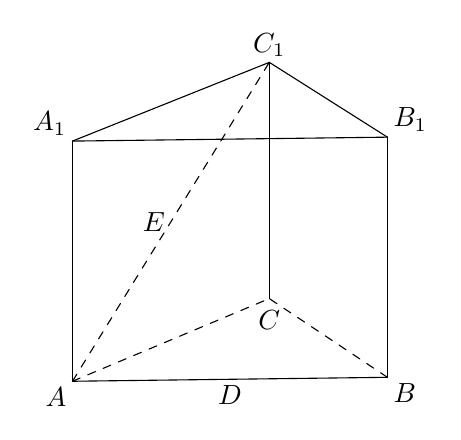
\begin{tikzpicture}[scale=1, line cap=round, line join=round]    % 三棱柱顶点    
\coordinate (C)  at (0.5, 0);   
 \coordinate (A)  at (-2.0, -1.05);   
 \coordinate (B)  at (2.0, -1.0);    
\coordinate (C1) at (0.5, 3.0);    
\coordinate (A1) at (-2.0, 2.0);   
 \coordinate (B1) at (2.0, 2.05);        % 特殊点    
\coordinate (D)  at (0, -1.025);    % AB 中点   
 \coordinate (E)  at (-0.75, 0.975); % AC₁ 中点
    % 不可见棱及辅助线(虚线)    
\draw[dashed] (A) -- (C);    
\draw[dashed] (B) -- (C);   
 \draw[dashed] (A) -- (C1);  % 体对角线 AC₁(经过 E)
    % 可见棱(实线)   
 \draw (A)  -- (B);    
\draw (A)  -- (A1);    
\draw (B)  -- (B1);   
 \draw (C)  -- (C1);   
 \draw (A1) -- (B1);   
 \draw (A1) -- (C1);   
 \draw (B1) -- (C1);
    % 标签(无小圆点)   
 \node[below left,  inner sep=2pt] at (A)  {$A$};    
\node[below right, inner sep=2pt] at (B)  {$B$};   
 \node[below,       inner sep=4pt] at (C)  {$C$};    
\node[above left,  inner sep=2pt] at (A1) {$A_1$};    
\node[above right, inner sep=2pt] at (B1) {$B_1$};   
 \node[above,       inner sep=2pt] at (C1) {$C_1$};   
 \node[below,       inner sep=2pt] at (D)  {$D$};   
 \node[left,        inner sep=2pt] at (E)  {$E$};
\end{tikzpicture}

（1）证明：$ DE\mathop{//} $ 平面 $ BCC_1B_1 $；

（2）设 $ CC_1=2 $，直线 $ DE $ 与平面 $ ACC_1A_1 $ 所成的角为 $ 45^\circ $，求直线 $ DE $ 到平面 $ BCC_1B_1 $ 的距离.
\end{problem}

\begin{answer}

\end{answer}

\begin{solutions}

\end{solutions}